\documentclass[11pt]{standalone}
\usepackage{amssymb}
\usepackage{amsmath}
\usepackage[no-math]{fontspec}
\usepackage{unicode-math}
\usepackage{libertinus}
\usepackage{pgf,xcolor}
\usepackage{tikz}
\usetikzlibrary{arrows.meta, backgrounds, calc}
\usepackage{pgfplots}
\pgfplotsset{compat=newest}

\definecolor{my_darkgray}{HTML}{484949}
\definecolor{my_lightgray}{HTML}{F3F4F4}
\definecolor{my_darkblue}{HTML}{005A94}
\definecolor{my_lightblue}{HTML}{CCDEE9}
\definecolor{my_yellow}{HTML}{FFEC7F}
\definecolor{my_red}{HTML}{E60000}
\definecolor{my_orange}{HTML}{E87846}

\begin{document}
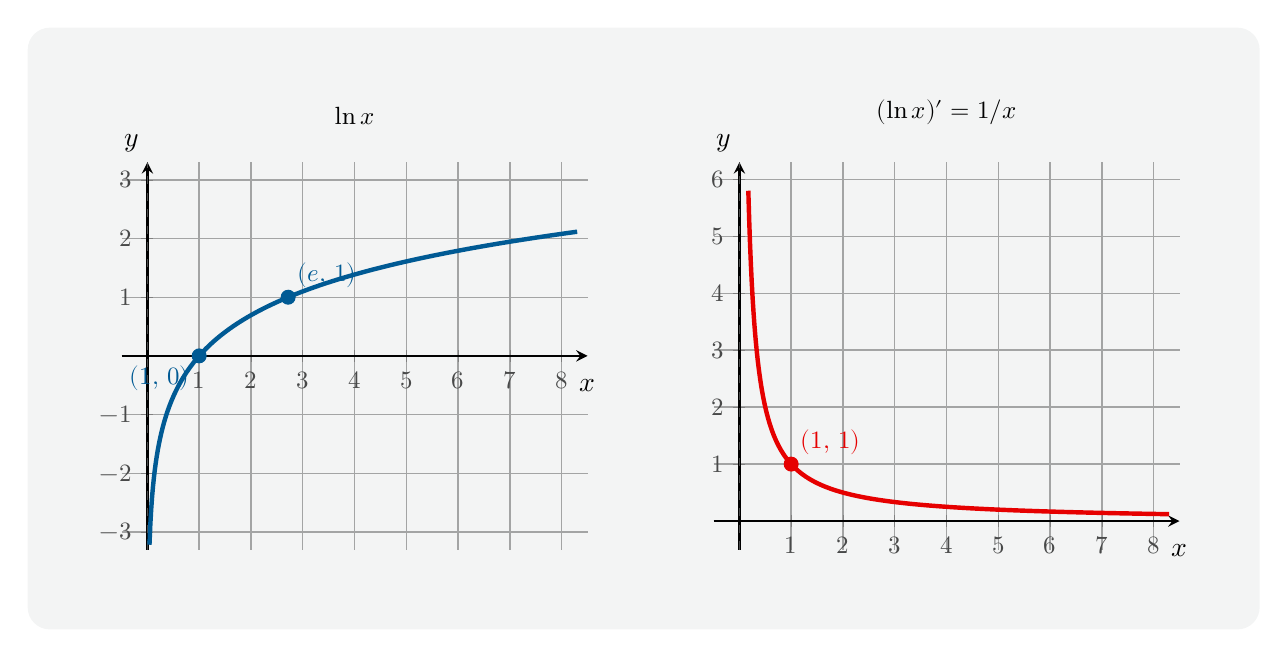
\begin{tikzpicture}[
    show background rectangle,
    background rectangle/.style={fill=my_lightgray, rounded corners=8pt},
    inner frame sep=0.8cm
]

% ── Left plot: ln(x) ────────────────────────────────────────────────────────
% Domain: x > 0. Vertical asymptote at x = 0.
% ln(1) = 0 is marked; ln(e) = 1 ≈ ln(2.718) is annotated.
\begin{axis}[
    name=left plot,
    axis lines = center,
    xlabel = {$x$},
    ylabel = {$y$},
    xlabel style = {at={(axis cs:8.5,0)}, anchor=north, yshift=-5pt},
    ylabel style = {anchor=south east},
    title = {$\ln x$},
    title style = {font=\small, text=black, yshift=4pt},
    grid = both,
    grid style = {line width=0.3pt, draw=my_darkgray!30},
    major grid style = {line width=0.5pt, draw=my_darkgray!50},
    % axis equal omitted: y range ±3 vs x range 0..8 – equal scaling would
    % compress the characteristic slow growth of the logarithm
    axis line style = {thick},
    xmin = -0.5, xmax = 8.5,
    ymin = -3.3, ymax = 3.3,
    xtick = {0,1,2,3,4,5,6,7,8},
    ytick = {-3,-2,-1,0,1,2,3},
    yticklabel style = {
        /pgf/number format/fixed,
        /pgf/number format/precision=0,
        font=\small,
        text=my_darkgray
    },
    xticklabel style = {font=\small, text=my_darkgray},
    width=7.5cm, height=6.5cm,
    clip=true,
]

% Vertical asymptote at x = 0
\addplot[draw=my_darkgray, dashed, thin]
    coordinates {(0,-3.3) (0,3.3)};

% ln(x), domain kept away from 0 to avoid log(0); restrict y as safety net
\addplot[
    draw=my_darkblue,
    samples=500,
    ultra thick,
    domain=0.04:8.3,
    restrict y to domain=-3.3:3.3
]{ ln(x) };

% Mark ln(1) = 0
\addplot[
    mark=*,
    mark size=2.5pt,
    only marks,
    draw=my_darkblue,
    fill=my_darkblue
] coordinates {(1, 0)};
\node[anchor=north east, font=\small, text=my_darkblue]
    at (axis cs:1, 0) {$(1,\,0)$};

% Mark ln(e) = 1 at x = e ≈ 2.718
\addplot[
    mark=*,
    mark size=2.5pt,
    only marks,
    draw=my_darkblue,
    fill=my_darkblue
] coordinates {(2.71828, 1)};
\node[anchor=south west, font=\small, text=my_darkblue]
    at (axis cs:2.71828, 1) {$(e,\,1)$};

\end{axis}

% ── Right plot: 1/x ─────────────────────────────────────────────────────────
% Domain: x > 0. 1/x diverges as x → 0⁺ and decays toward 0 as x → ∞.
% The value (1/x)|_{x=1} = 1 matches the slope of ln(x) at x = 1.
\begin{axis}[
    name=right plot,
    at={($(left plot.east)+(1.6cm,0)$)},
    anchor=west,
    axis lines = center,
    xlabel = {$x$},
    ylabel = {$y$},
    xlabel style = {at={(axis cs:8.5,0)}, anchor=north, yshift=-5pt},
    ylabel style = {anchor=south east},
    title = {$(\ln x)' = 1/x$},
    title style = {font=\small, text=black, yshift=4pt},
    grid = both,
    grid style = {line width=0.3pt, draw=my_darkgray!30},
    major grid style = {line width=0.5pt, draw=my_darkgray!50},
    % axis equal omitted: y range 0..6 vs x range 0..8 – equal scaling would
    % make the steep rise near x = 0 appear nearly vertical and unreadable
    axis line style = {thick},
    xmin = -0.5, xmax = 8.5,
    ymin = -0.5, ymax = 6.3,
    xtick = {0,1,2,3,4,5,6,7,8},
    ytick = {0,1,2,3,4,5,6},
    yticklabel style = {
        /pgf/number format/fixed,
        /pgf/number format/precision=0,
        font=\small,
        text=my_darkgray
    },
    xticklabel style = {font=\small, text=my_darkgray},
    width=7.5cm, height=6.5cm,
    clip=true,
]

% Vertical asymptote at x = 0
\addplot[draw=my_darkgray, dashed, thin]
    coordinates {(0,-0.5) (0,6.3)};

% 1/x for x > 0; restrict y to domain guards against blow-up near x = 0
\addplot[
    draw=my_red,
    samples=500,
    ultra thick,
    domain=0.04:8.3,
    restrict y to domain=0:6.3
]{ 1/x };

% Mark (1, 1): derivative of ln(x) at x = 1 equals 1
\addplot[
    mark=*,
    mark size=2.5pt,
    only marks,
    draw=my_red,
    fill=my_red
] coordinates {(1, 1)};
\node[anchor=south west, font=\small, text=my_red]
    at (axis cs:1, 1) {$(1,\,1)$};

\end{axis}

\end{tikzpicture}
\end{document}
